%%%%%%%%%%%%%%%%%%%%%%%%%%%%%%%%%%%%%%%%%%%%%%%%%%%%%%%%%%%%%%%%%%%%%%
% writeLaTeX Example: A quick guide to LaTeX
%
% Source: Dave Richeson (divisbyzero.com), Dickinson College
% 
% A one-size-fits-all LaTeX cheat sheet. Kept to two pages, so it 
% can be printed (double-sided) on one piece of paper
% 
% Feel free to distribute this example, but please keep the referral
% to divisbyzero.com
% 
%%%%%%%%%%%%%%%%%%%%%%%%%%%%%%%%%%%%%%%%%%%%%%%%%%%%%%%%%%%%%%%%%%%%%%
% How to use writeLaTeX: 
%
% You edit the source code here on the left, and the preview on the
% right shows you the result within a few seconds.
%
% Bookmark this page and share the URL with your co-authors. They can
% edit at the same time!
%
% You can upload figures, bibliographies, custom classes and
% styles using the files menu.
%
% If you're new to LaTeX, the wikibook is a great place to start:
% http://en.wikibooks.org/wiki/LaTeX
%
%%%%%%%%%%%%%%%%%%%%%%%%%%%%%%%%%%%%%%%%%%%%%%%%%%%%%%%%%%%%%%%%%%%%%%

\documentclass[10pt,landscape]{article}
\usepackage{amssymb,amsmath,amsthm,amsfonts,bm}
\usepackage{multicol,multirow}
\usepackage{calc}
\usepackage{ifthen}
\usepackage[landscape]{geometry}
\usepackage[colorlinks=true,citecolor=blue,linkcolor=blue]{hyperref}
\usepackage{graphicx}
\graphicspath{ {./images/} }

\ifthenelse{\lengthtest { \paperwidth = 11in}}
    { \geometry{top=.5in,left=.5in,right=.5in,bottom=.5in} }
	{\ifthenelse{ \lengthtest{ \paperwidth = 297mm}}
		{\geometry{top=1cm,left=1cm,right=1cm,bottom=1cm} }
		{\geometry{top=1cm,left=1cm,right=1cm,bottom=1cm} }
	}
\pagestyle{empty}
\makeatletter
\renewcommand{\section}{\@startsection{section}{1}{0mm}%
                                {-1ex plus -.5ex minus -.2ex}%
                                {0.5ex plus .2ex}%x
                                {\normalfont\large\bfseries}}
\renewcommand{\subsection}{\@startsection{subsection}{2}{0mm}%
                                {-1explus -.5ex minus -.2ex}%
                                {0.5ex plus .2ex}%
                                {\normalfont\normalsize\bfseries}}
\renewcommand{\subsubsection}{\@startsection{subsubsection}{3}{0mm}%
                                {-1ex plus -.5ex minus -.2ex}%
                                {1ex plus .2ex}%
                                {\normalfont\small\bfseries}}
\makeatother
\setcounter{secnumdepth}{0}
\setlength{\parindent}{0pt}
\setlength{\parskip}{0pt plus 0.5ex}
% -----------------------------------------------------------------------

\title{ROB501 Cheat Sheet}

\begin{document}

\raggedright
\footnotesize

\begin{multicols}{3}
\setlength{\premulticols}{1pt}
\setlength{\postmulticols}{1pt}
\setlength{\multicolsep}{1pt}
\setlength{\columnsep}{2pt}

\section{L1 Introduction}
\textbf{inverse problem}: recover unknown parameters from insufficient information to identify/bound the solution (need phy/prob/assumptions), find/bound unknowns (sol’n), otherwise \textbf{Forward}, e.g. rendering

\textbf{Well-posed}:  a unique solution exists, changes continuously with the initial conditions

vision problems are \textbf{ill-posed} b/c 2D-3D not unique

\textbf{image function}: $I = \mathcal{P}(G, M, V, L, A, \epsilon)$, $(G, M, V) = \mathcal{P}^{-1}(I) + \text{other sensors, knowledge, experience, etc}$, with Geometry, Materials, Viewpoint, Lighting, Atmospherics, Noise+distractors

Geometry(3D, 4D) vs Appearance(2D projection)

Moravec's Paradox: high-level reasoning requires little computation, while low-level sensorimotor processing requires tremendous resources.

\section{L2 Mathematical Fundamentals}
Geometric (points, lines) and Photometric (brightness, contrast) are intertwined

Reference frame ($\underset{\rightarrow}{\mathcal{F}}_v$): physical reference points uniquely fixing (locate and orient) a coordinate system

2D Homogeneous form of points: $\bm{\Tilde{x}} = (\Tilde{x}, \Tilde{y}, \Tilde{w})\in \mathcal{P}^2 \triangleq R^3 \backslash (0,0,0)$ ($\mathcal{P}$ is projective space), back to 2D Inhomogeneous form $\mathbf{\Tilde{x}} = \Tilde{w}(x, y, 1) = \Tilde{w}\mathbf{\Bar{x}}$, 2D augmented vector:  $\mathbf{\Bar{x}} = (x, y, 1)$

$\Tilde{w}=0$ are ideal pts/pts at infinity/where 2 parallel lines intersect/no inhomogeneous form (so $P^2$ has more pts than $R^2$)

2D Homo. form of lines: $\Tilde{\mathbf{l}} = (a,b,c)$, corresponding eqn: $\Bar{\mathbf{x}}\cdot \Tilde{\mathbf{l}} = ax + by +c=0$, $\mathbf{l}=(\hat{n}_x, \hat{n}_y,d) = (\hat{n}, d)$, $\hat{n}$ normal vector, $d$ distance to origin

Points vs Lines: $\Tilde{l} = \Tilde{x}_1 \times \Tilde{x}_2$, $\Tilde{x} = \Tilde{l}_1 \times \Tilde{l}_2$

Cross product: $||\mathbf{u} \times \mathbf{v}|| = ||u||||v||sin\theta$, $\mathbf{u} \times \mathbf{v} = [u]_\times v = \begin{bmatrix} u_2v_3-v_2u_3 & u_3v_1-v_3u_1 & u_1u_2-v_1v_2\end{bmatrix}^T$ where $[u]_\times^T = -[u]_\times$, $[u]_x \triangleq \begin{bmatrix} 0 & -u_3 & u_2 \\ u_3 & 0 & -u_1 \\ -u_2 & u_1 & 0\end{bmatrix}$

Active transform = point coord. change

Transformation in 2D

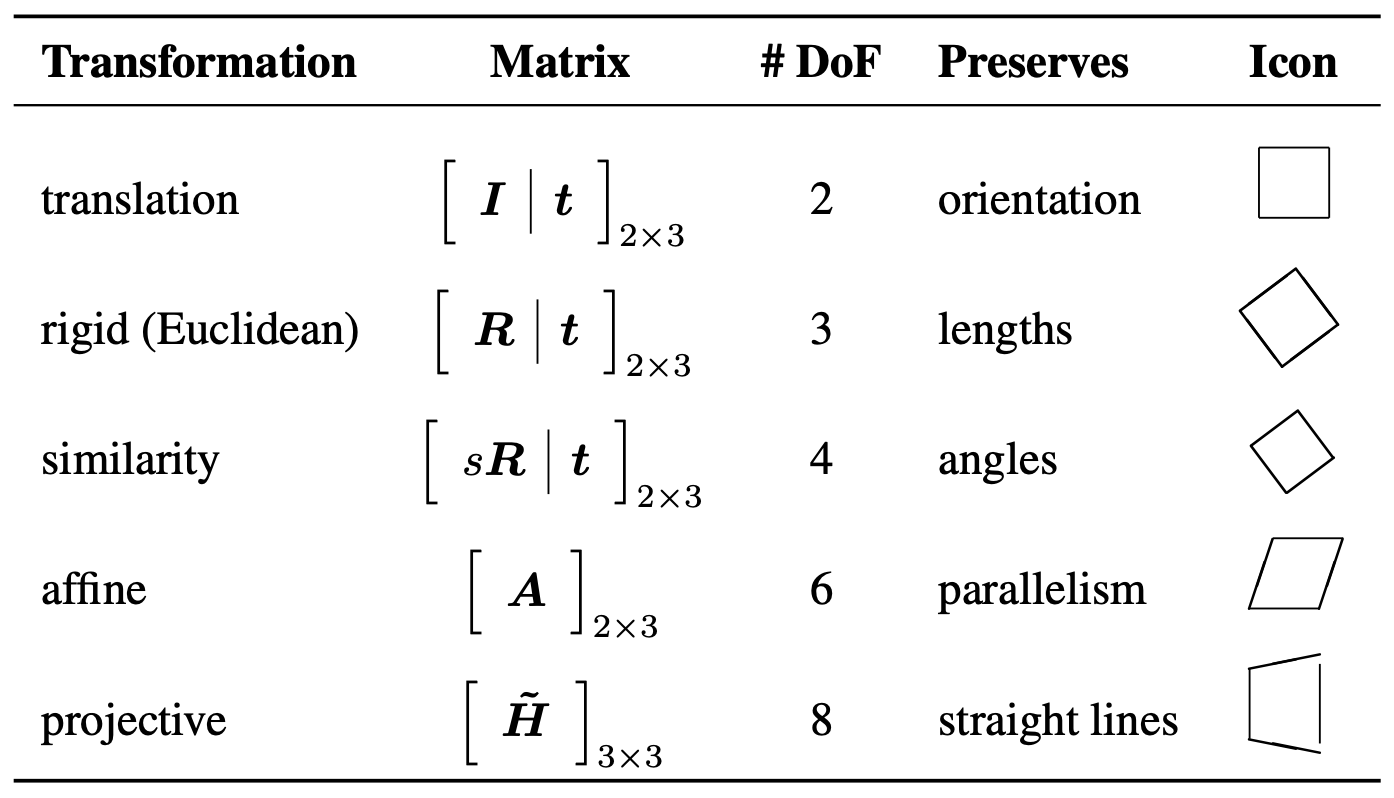
\includegraphics[width=6cm]{images/trans_2d}

1. Euler’s Angle (eg. yaw-pitch-roll=z-y-x=$\mathbf{C}(\psi)\mathbf{C}(\theta)\mathbf{C}(\phi)$) Singularity when $\theta = \pi/2$.

2. Axis-Angle (Rodriguez's formula): $\mathbf{C}(\hat{\mathbf{n}}, \theta) = \mathbf{I}_3 + sin\theta [\hat{\mathbf{n}}]_\times + (1-cos\theta)[\hat{\mathbf{n}}]^2_\times$

3. Quaternions($\mathbb{H}$)
$\bm{q} = q_0 + \mathbf{q} = q_0 + q_1\hat{\mathbf{i}} + q_2\hat{\mathbf{j}} + q_3\hat{\mathbf{k}}$, $i^2 =j^2=k^2=ijk=-1$. Unit quaternions $\mathbb{S}^3 = \{\bm{q}\in \mathbb{H} | ||\bm{q}^2 = q_0^2 + q_1^2 + q_2^2 + q_3^2=1||\}$, $\bm{q} = \begin{bmatrix} q_0 \mathbf{q}\end{bmatrix} = \begin{bmatrix} cos(\theta/2) \\ \hat{\mathbf{u}}sin(\theta/2)\end{bmatrix}$, $\mathbf{C}(\hat{\mathbf{n}}, \theta) = \mathbf{I}_3 + 2q_0[\mathbf{q}]_\times + 2[\mathbf{q}]_\times^2$, $\bm{p}\oplus\bm{q} = (p_0+\mathbf{p}) \oplus (q_0+\mathbf{q}) = p_0q_0-\mathbf{p}^T\mathbf{q}+p_0\mathbf{q}+q_0\mathbf{p}+\mathbf{p}\times\mathbf{q}$



\section{L3 Probability Theory and Estimation Techniques}
Posterior = likelihood * prior / evidence

Expectation $E(f(x)) = \sum_xf(x)p(x)$ or $\int_x f(x)p(x)dx$

Gaussian(normal): $X \sim \mathcal{N}(\mu,\,\sigma^{2}) = \dfrac{1}{\sqrt{2\sigma^2\pi}}e^{-\dfrac{(x-\mu)^2}{2\sigma^2}}$
$\mathbf{x}\sim \mathcal{N}(\mathbf{\mu},\,\mathbf{\Sigma}) = 2\pi^{-\frac{n}{2}}det\Sigma^{-\frac{1}{2}}e^{-\frac{1}{2}(\mathbf{x} - \mathbf{\mu})^T\Sigma^{-1}(\mathbf{x} - \mathbf{\mu})}$

Estimation when overdetermined (\#pts/epns > \#parameters), e.g.  linear least sq/regress: $\theta =(m,b)$, minimize sum of residuals’ square: $E_{WLS} = \sum_i w_i||\Tilde{y}_i - \mathbf{J}(x_i)\mathbf{\theta}||^2$

$\hat{\theta} = [\sum_i \mathbf{J}^T(x_i)W\mathbf{J}(x_i)]^{-1}[\mathbf{J}^T(x_i)\Tilde{y}_i]$, $w=\sigma_i^{-2}$

Outlier: observation distant from others, due to measurement variability/error - sol’n: RAndom SAmple Consensus RANSAC:

1. Min \# data pts needed to fit model\par
2. Try $k$ random subsets  of \# \par
3. Count $x$ of them are within error tolerance threshold ($t$)?\par
4. If x is above threshold of “at least $n$ compatible pts” -> terminate, or repeat till $n$ or $k$
Params: $k, n, t$

$E[k] = b(1 + 2a + 3a^2 + ... + ia^{i-1}+...) = 1/b = w^{-n}$ where, $b = w^n, a = (1-b)$, $w$ prob of not outlier.
$Z = P{\text{(}\geq \text{1 selection is good})=1- (1-w^n)^k = 1 - (1-b)^k}$, $k=\frac{log(1-z)}{log(1-b)}$

\section{L4 Image Formation and Optics}
Camera obscura/Pinhole camera: aperture size decreases, images are sharper \& dimmer.\\
\textbf{(scaled) orthography projection}: drop the z to get 3D -> 2D, good for long focal length, $\Tilde{x} = \begin{bmatrix} 1 & 0 & 0 & 0 \\ 0 & 1 & 0 & 0 \\ 0 & 0 & 0 & 1\end{bmatrix}\Tilde{p}$

Ideal pinhole: aperture=single pt. All light rays intersect at the \textbf{optic center}, origin of the camera frame.\\
\textbf{Optical axis} pierces the image plane at the \textbf{principal point} and 
\textbf{optic center}
landmark point $p = (x,y,z) $ to image plane: projective map:
$\Bar{x} = \mathcal{P}_z(\mathbf{p}) = [x/z, y/z, 1]^T$: normalized image plane coord. (Similar triangles)\\
Field of View $\theta$: $tan\frac{\theta}{2} = \frac{W}{2f}$, f: focal length, W: Sensor width\\
Intrinsic params. matrix $\mathbf{K}$: principal pt. at $(c_x, c_y)$, skew, focal length (affine w/ 5 parameters)\\
 $\begin{bmatrix} x_s \\ y_s \\ 1\end{bmatrix} = \begin{bmatrix} f_x & s & c_x \\ 0 & f_y & c_y \\ 0 & 0 & 1\end{bmatrix}\begin{bmatrix} x/z \\ y/z \\ 1\end{bmatrix} = \mathbf{K}\dfrac{\mathbf{p}}{z}$

Extrinsic params. matrix $\mathbf{E}=[\mathbf{C}|\mathbf{t}]$. ($\mathbf{E}_{cw}$ is world to camera)

Together:
$\mathbf{\Tilde{P}} = \begin{bmatrix} \mathbf{K} & 0 \\ \mathbf{0}^T & 1\end{bmatrix}\begin{bmatrix} \mathbf{C} & \mathbf{t} \\ \mathbf{0}^T & 1\end{bmatrix} = \Tilde{\mathbf{K}}\mathbf{E}$

Augmented $p_w = (x_w, y_w, z_w, 1)$ in world to $x_s = (x_s, y_s, 1, d)$ on image, with $\Tilde{x}_s = \Tilde{P}\Bar{p}_w$ divided by 3rd elem $z$, $d=1/z=1/(C_zp_w+t_z)$

Lens distortion (aperture != a pt)
\textbf{Radial} (from \textbf{centre of distortion}, Barrel vs.Pincushion) + \textbf{Tangential} (tilting of img plane) = \textbf{plumb bob model}: $\begin{bmatrix} x_d \\ y_d \end{bmatrix} = (1 + \kappa r^2 + \kappa_2 r^4 + \kappa_3 r^6)\begin{bmatrix} x_n \\ y_n \end{bmatrix} + \begin{bmatrix} 2\tau_1 x_ny_n + \tau_2(r^2 + 2x_n^2) \\ 2\tau_2 x_ny_n + \tau_1(r^2 + 2y_n^2) \end{bmatrix}$

Image unwarping: no analytical solution (inverse of distortion), so precompute a nonlinear transform to unwarp:  find distorted coordinates from normalized ones, bilinear interpolation

From world to image plane
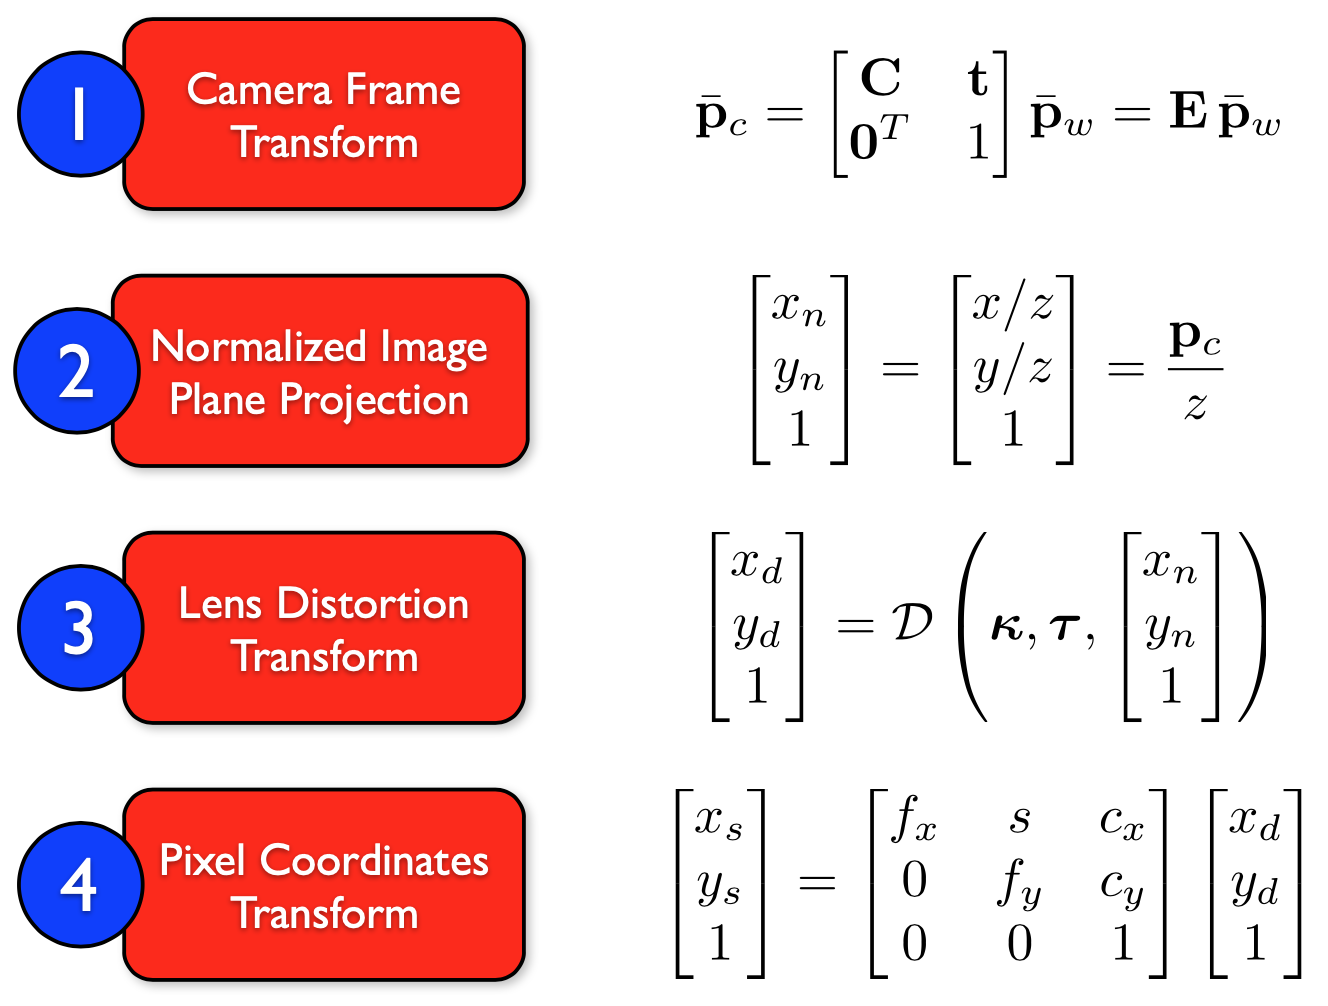
\includegraphics[width=6cm]{images/world_to_image.png}

Alternative model (other than plumb bob): fisheye, omni-directional, catadioptric (involves both the reflecting and refracting)

Lens Optical Effects:
1.\textbf{Chromatic aberration}: different colours ($\lambda$) focus at different distances (diff f to diff z) \& magnification - per-color radial distort 
2.\textbf{Vignetting}: darker towards edge, due to fore-shortening(visual compression of an image) of surface, lens aperture ($cos^4$ model)

Digital Camera sensors:\\
CCD (accumulate photons and then use 'bucket brigade' charge readout)\\
CMOS (measures photons using conductivity changes)\\

spatial sampling (may cause aliasing): need $f_s \geq 2f_{max}$

Colour Cameras and Filter Arrays, from 3 (RGB) to filter on top - Bayer Mosaics

\section{L5 Image Processing and Transformations}

\textbf{Point operation}

(1) \textbf{Per-pixel transform}: 
e.g. thresholding, brightness adjustment, contrast adjustment, gamma correction\\
may require global information
General image processing operator: $g(x) = h(f_0(x), ..., f_n(x))$,\\
discrete: $\text{pixel location} x = (i,j), g(i,j) = h(f(i,j)).$ \\

1. $g(x)=a(x)f(x)+b(x), a=gain, b=bias$
2. $g(x)=f(x)^{1/\gamma}$, gamma correction to remove nonlinear radiance map\\

(2) \textbf{Histogram}: lookup table of \# pixels with a grey level value vs. Level  (usually  $r_k \in [0, L-1=255]$). Normalized , $p(r_k) = n_k/n$: prob of $r_k$’s occurrence, $n$:total \# pixel\\
Hist. Equaliz’n: intensity mapping func. $s_k = T(r_k) = \sum_{j=0}^k p_r(r_j) = \sum_{j=0}^k \dfrac{n_j}{n}, k=0,..L-1$

\textbf{Neighbourhood op}

\textbf{Linear filtering}: convolution $g=f*h$, padding: zero, constant, clamp/replicate, cyclic wrap, and mirror

\textbf{Separable Lin. filter}: General size $K$ kernel conv. needs $K^2$ op per pixel. Separable: 2D $K=vh^T$, 1D horizontal $h$ then 1D vertical $v$ s.t only $2K$ op. Inspect or if SVD’s 1st $\sigma \neq 0$. Isotropic Gaussian kernel is separable.

Gaussian filter: $G(x, y; \sigma) = \dfrac{1}{2\pi \sigma^2}e^{-\frac{x^2 + y^2}{2\sigma^2}}$

Band-pass filter (LoG, DoG) remove high & low freq, LoG used for edge detection, LoG (scale-space properties): $\nabla^2G(x,y;\sigma) = \dfrac{\partial^2G}{dx^2}+\dfrac{\partial^2G}{dy^2}=\dfrac{x^2 + y^2 + 2\sigma^2}{\sigma^4}G(x,y;\sigma)$

\textbf{Integral image/ summed area table:}$s(i,j) =\sum_{k=0}^i\sum_{l=0}^{j}f(k,l)= s(i-1,j)+s(i,j-1)-s(i-1,j-1)+s(i,j)$

\textbf{Nonlinear filter}: median filter, $\alpha$-trimmed median(exclude $\alpha$ extremes), min and max filters, and bilateral filter.

\textbf{Geometric transform} $g(x)=f(h(x))$:
1. Forward $x’=h(x)$, copy pixel $f(x)$ to $g(x’)$, but non-integer $x’$ causes aliasing and blur even with bilinear interpolation. 
2. Inverse $x=\hat{h}(x’)$ (with inverse matrix), interpolate $x$ from original img to copy to integer $x’$.

\textbf{Regularization} of ill-posed (often ill-conditioned) inverse problem
$\epsilon_d = \int\int f_x^2(x,y) + f_y^2(x,Y)dxdy = \int\int||\nabla f(x,y)||^2dxdy$
$\epsilon_d = \int\int (f(x,y) - d(x,y))^2dxdy$
minimize $\epsilon=\epsilon_d + \lambda \epsilon_1$, $\lambda$ control smooth 

\section{L6 Image Features Detection and Description}
Feature: Salient (distinctive), Local (small subset of pixels), Repeatable (stable in time space), Compact (math-wise) region

Matching (criteria): find correspondence

Match two patch: $E_{WSSD}(\mathbf{u} = \sum w(\mathbf{x}_i) (I_1(\mathbf{x}_i + \mathbf{u}) - I_0(\mathbf{x}_i))^2)$

$E_{AC}(\mathbf{\nabla u}) = \sum w(\mathbf{x}_i) (I_1(\mathbf{x}_i + \mathbf{\nabla u}) - I_0(\mathbf{x}_i))^2)\approx \sum_i w(\mathbf{x}_i) (\nabla I_0(x_i)\cdot\Delta\mathbf{u})^2 =  \Delta\mathbf{u}^T\mathbf{A}\Delta\mathbf{u}$, $\mathbf{A} = w * \begin{bmatrix} I_x^2 & I_xI_y \\ I_xI_y & I^2_y\end{bmatrix}$

Image gradient: $\nabla I_0(\mathbf{x}_i) = (\dfrac{\partial I_0}{\partial x}, \dfrac{\partial I_0}{\partial y})(\mathbf{x}_i)$

\textbf{Harris}: $det \mathbf{A} - \alpha trace \mathbf{A}^2 = \lambda_0\lambda_1 - \alpha(\lambda_0+ \lambda_1)$ rotation/bias invariant, but gain/scale will affect.

\textbf{SIFT} - location \& scale-invariant
\textbf{Step 1}. Get \textbf{scale space} by Gaussian filter (down-sample by 2 each time)
\textbf{Step 2}. Find keypoints w/ DoG (handle scale) for LoG (don't handle scale)
\textbf{Step 3}. Reject asymmetry curvatures (only keep corner)
\textbf{Step 4}. Assign orientation
\textbf{Step 5}. Final descriptor
(4x4 grid with 8-orientation(8-bins) gives 128D vector)

\section{L7 Image Features Matching and Tracking}
Matching approach - distance func
1. SSD (threshold or ratio)
3. Euclidean dist. (SIFT/SURF), \& threshold
4. Hamming dist. (BRISK) for dissimilarity

Confusion matrix: measures matching performance (func of threshold). 
\textbf{TP}: correct match, 
\textbf{FN}: incorrectly rejected, 
\textbf{FP}: incorrectly matched, 
\textbf{TN}: correctly rejected. 
\textbf{TODO} Confusion matrix
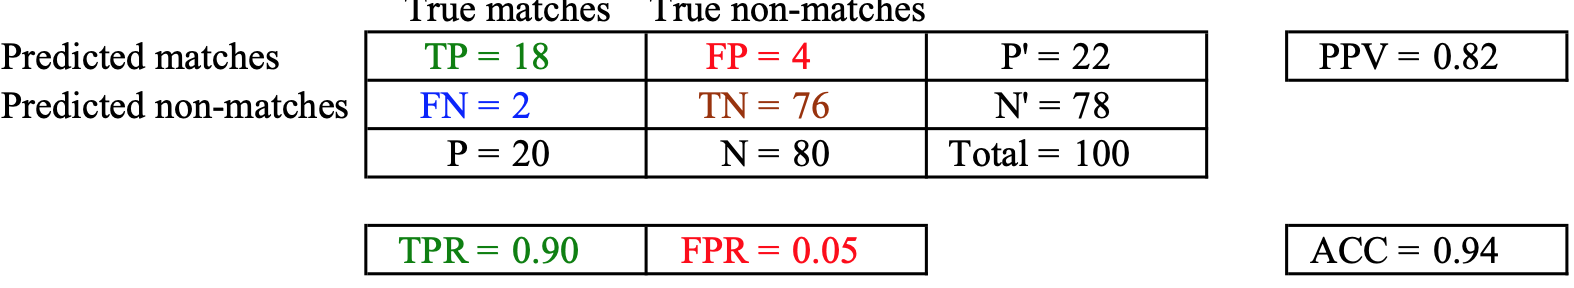
\includegraphics[width=6cm]{images/confusion_mtx.png}

Receiver operating characteristic curve
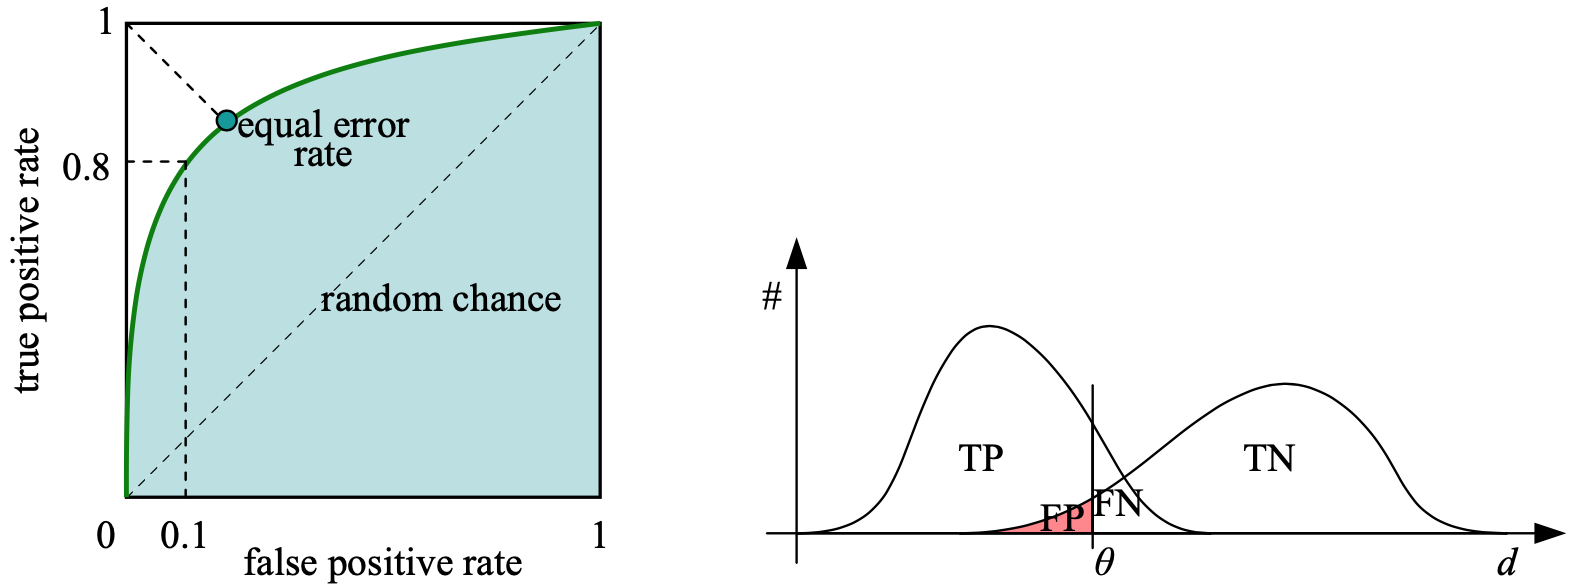
\includegraphics[width=6cm]{images/roc.png}

\textbf{TPR} = TP / (TP+FN)TP/P
\textbf{FPR}=FP/(FP+TN)=FP/N
\textbf{PPV}=TP/(TP+FP)=TP/P'
\textbf{ACC}=(TP+TN)/(P+N)

Feature mapping -
1. Compare all $O(n^2)$
2. Search spatially close features
3. Hash table/vocab tree in feat. space
4. Multidimentional k-d tree

5. Tracking incrementally: find a set of likely feature loc in 1st img, search for corresponding locations in subsequent imgs.
Good cond:
1. Limited motion & scene deformation,
2. Good feature to track (same as good-for-matching, or low SSD, or normalized cross-correlation)
If not good cond: use \textbf{multi-resolution search} or a \textbf{predictive model}.

KLT tracker: keep measures of feature dissimilarity between current vs. 1st frame in sequence; discard when dissimilarity grows too large (RMS residual)  w/ an affine motion model to warp imgs’ deformation back to 1st frame

\section{L8 Camera Pose Estimation}
Pose Estimation = Object pose + camera pose (extrinsic calibration(min 3 pts (+ 3 for $K$)), P3P, PnP)

Gaussian Newton Optimization \textbf{TODO}

Solve constraints on rotation matrix \textbf{TODO}
initial point (from DLT) is important. no constraints (on vector space). Gauss-Newton approximately fits a quadratic cost.

\section{L9 Stereo Vision}
Stereo-vision: The \textbf{baseline} between the left and right optical centres provides \textbf{parallax}.

Stereo-matching \textbf{TODO}

Rectification: result in \textbf{fronto-parallel} or \textbf{standard rectified} image, \textbf{TODO}

Disparity (after rectification): difference between the coordinates of the matching points (patches) in both images. In (left) camera frame: $Z = \dfrac{bf}{d}$, $Z$ depth, $b$ baseline, $f$ focal length, $d$ disparity

Stereo camera model: $\begin{bmatrix} x_0 \\ y_0 \\ d\end{bmatrix} = \mathbf{f}(\mathbf{p}_c)=\dfrac{f}{Z}\begin{bmatrix} X \\ Y \\ b\end{bmatrix} + \begin{bmatrix} c_x \\ c_y \\ 0\end{bmatrix}$

Distance is inversely proportional to the absolute value of the disparity; Disparity is directly proportional to the baseline of the stereo array
for long-range stereo, \textbf{subpixel disparity}

Dense Stereo Correspondence - Local (Window based) Correspondence Algorithms

Similarity measure (SAD, SSD), aggregation (convolution), find the ‘best’ match;

For wide baselines, \textbf{foreshortening} of objects often causes matching to fail (a fixed window size cannot account for perspective change).

\section{L10 Monocular and Stereo Camera Calibration}
N-Planes Calibration (intrinsic parameters and lens distortion coefficients)

Critically important to include a variety of views, with target at multiple angles and distances, and fully covering entire image plane (over several views) to properly constrain/estimate calibration parameters

Why a checkboard?
The effect of perspective projection on the cross-junctions (see Project #2) of a checkerboard target can be easily determined (i.e., the amount of foreshortening)
For circles, the foreshortening effect is more complex, and the centre of the warped ellipse is not the same as the projected centre of the original circle
\textbf{TODO}

Stereo Camera Calibration
Stereo calibration is a straightforward extension of monocular calibration, typically using the same target-based approach
An additional 3D rigid-body transform between the cameras is added to the optimization parameter vector
Optimization depends on observation of the same features (e.g., target corner points) from both cameras (and features must be matched)

\section{L11 Structure from Motion, Bundle Adjustment}

The SfM Problem
Structure from Motion (or SfM) is the problem of determining both the 
 3D positions of landmark points (structure) and a series of camera poses (motion) from a set of sparse image feature correspondences

Triangulation involves finding the 3D position of a landmark point from a set of image correspondences and known camera poses

$\mathbf{v}_j = \mathbf{C}_j^{-1}\mathbf{K}_j^{-1}$ (unnormalized), $e(x) = c_j + d_j\mathbf{v}_j-\mathbf{p}$, $d_j = \mathbf{v}_j \cdot (\mathbf{p} - \mathbf{c}_j)$, optical center in world frame $\mathbf{c}_j$, $\mathbf{q}_j = \mathbf{c}_j + (\mathbf{v}\mathbf{v}^T)(\mathbf{p}-\mathbf{c}_j)$

\textbf{Bundle adjustment} is “is the problem of refining a visual reconstruction to produce jointly optimal 3D structure and viewing parameter estimates”

Viewing parameters include camera poses and/or calibration coefficients • Optimal is with respect to a given cost function, and jointly implies
simultaneous optimality over both structure and camera variations

M-estimators for outliers

Structure and Sparsity

Naive implementation of nonlinear least squares (the common solution method) is \textbf{cubic in the number of parameters} involved
• Most adjustment computations involve sparse matrices (i.e., the Jacobian
is sparse, and also the Hessian), and this can be exploited
\textbf{Incremental updates} sparse Cholesky factorization (matrix square root)
• Global parameters (common to all cameras, e.g., intrinsics or stereo rig configuration) should be ordered last to reduce fill-in
\textbf{TODO}

Alternatives Methods and Implementation Details
Incremental update methods: extended Kalman filter, a standard estimation tool that operates sequentially
A variety of techniques are available for the full problem that attempt to reduce the computational complexity: Fixed (sliding) window adjustment, where only parameters in the window are optimized

Keyframe-based algorithms, which select a subset of ‘relevant’ frames to adjust (used in many SLAM systems)

• Often a good idea to use homogenous coordinates for the structure (landmark) parameters to avoid numerical instabilities for points near infinity

Bundle Parameterization
Points, the homogeneous projective parameterization $\mathbf{\Tilde{x}} = (\Tilde{x}, \Tilde{y}, \Tilde{z}, \Tilde{w})$
naturally incorporates points near infinity in a finite and well-conditioned way, maintaining numerical stability (although normalization is still needed)
• For rotations, it is best to use either quaternions (subject to a norm of one) as a global parameterization, or to use rotation matrices
Incremental local rotation updates can be made using any well-behaved, 3-parameter rotation parameterization
• Options include local Euler angles, Rodriguez parameters, modified Rodriguez parameters, etc.

Error Modelling in Adjustment

cost of outliers is down-weighted
• Note that accurate error modelling is at least important as accurate geometric modelling
Gaussian distributions have short tails, that is, the distributions fall off very quickly compared to more realistic error models
• Realistic long-tailed distributions are more suited for modelling



% \section{What is \LaTeX?}
% \LaTeX (usually pronounced ``LAY teck,'' sometimes ``LAH teck,'' and never ``LAY tex'') is a mathematics typesetting program that is the standard for most professional mathematics writing. It is based on the typesetting program \TeX\ created by Donald Knuth of Stanford University (his first version appeared in 1978). Leslie Lamport was responsible for creating \LaTeX\, a more user friendly version of \TeX. A team of \LaTeX\ programmers created the current version,  \LaTeX\ 2$\varepsilon$.

% \section{Math vs. text vs. functions}
% In properly typeset mathematics  variables appear in italics (e.g., $f(x)=x^{2}+2x-3$). The exception to this rule is predefined functions (e.g., $\sin (x)$). Thus it is important to \textbf{always} treat text, variables, and functions correctly. See the difference between $x$ and x, -1 and $-1$, and $sin(x)$ and $\sin(x)$.  

% There are two ways to present a mathematical expression--- \emph{inline} or as an \emph{equation}.

% \subsection{Inline mathematical expressions}
% Inline expressions occur in the middle of a sentence.  To produce an inline expression, place the math expression between dollar signs (\verb!$!).  For example, typing \verb!$90^{\circ}$ is the same as $\frac{\pi}{2}$ radians!  yields $90^{\circ}$ is the same as $\frac{\pi}{2}$ radians.

% \subsection{Equations}
% Equations are mathematical expressions that are given their own line and are centered on the page.  These are usually used for important equations that deserve to be showcased on their own line or for large equations that cannot fit inline. To produce an inline expression, place the mathematical expression  between the symbols  \verb!\[! and \verb!\]!. Typing \verb!\[x=\frac{-b\pm\sqrt{b^2-4ac}}{2a}\]! yields \[x=\frac{-b\pm\sqrt{b^2-4ac}}{2a}.\]
 
% \subsection{Displaystyle} 
% To get full-sized inline mathematical expressions  use  \verb!\displaystyle!. Use this sparingly. Typing \verb!I want this $\displaystyle \sum_{n=1}^{\infty}! \verb!\frac{1}{n}$, not this $\sum_{n=1}^{\infty}! \verb!\frac{1}{n}$.! yields\\ I want  this $\displaystyle \sum_{n=1}^{\infty}\frac{1}{n}$, not this $\sum_{n=1}^{\infty}\frac{1}{n}.$


% \section{Images}

% You can put images (pdf, png, jpg, or gif) in your document. They need to be in the same location as your .tex file when you compile the document. Omit   \verb![width=.5in]! if you want the image to be full-sized.

% \verb!\begin{figure}[ht]!\\
% \verb!\includegraphics[width=.5in]{imagename.jpg}!\\
% \verb!\caption{The (optional) caption goes here.}!\\
% \verb!\end{figure}!

% \subsection{Text decorations}

% Your text can be \textit{italics} (\verb!\textit{italics}!), \textbf{boldface} (\verb!\textbf{boldface}!), or \underline{underlined} (\verb!\underline{underlined}!).

% Your math can contain boldface, $\mathbf{R}$ (\verb!\mathbf{R}!), or blackboard bold, $\mathbb{R}$ (\verb!\mathbb{R}!). You may want to used these to express the sets of real numbers ($\mathbb{R}$ or $\mathbf{R}$), integers ($\mathbb{Z}$ or $\mathbf{Z}$), rational numbers ($\mathbb{Q}$ or $\mathbf{Q}$), and natural numbers ($\mathbb{N}$ or $\mathbf{N}$).

% To have text appear in a math expression use \verb!\text!. \verb!(0,1]=\{x\in\mathbb{R}:x>0\text{ and }x\le 1\}! yields $(0,1]=\{x\in\mathbb{R}:x>0\text{ and }x\le 1\}$. (Without the \verb!\text! command it treats ``and'' as three variables: $(0,1]=\{x\in\mathbb{R}:x>0 and x\le 1\}$.)



% \section{Spaces and new lines}

% \LaTeX\ ignores extra spaces and new lines. For example, 

% \verb!This   sentence will       look!

% \verb!fine after      it is     compiled.!

% This   sentence will       look
% fine after      it is     compiled.


% Leave one full empty line between two paragraphs. Place \verb!\\! at the end of a line to create a new line (but not create a new paragraph).

% \verb!This!

% \verb!compiles!

% ~

% \verb!like\\!

% \verb!this.!

% This
% compiles 

% like\\
% this.

% Use  \verb!\noindent! to prevent a paragraph from indenting.

% \section{Comments}

% Use \verb!%! to create a comment. Nothing on the line after the \verb!%! will be typeset. \verb!$f(x)=\sin(x)$ %this is the sine function! yields $f(x)=\sin(x)$%this is the sine function

% \section{Delimiters}

% \begin{tabular}{lll}
% \emph{description} & \emph{command} & \emph{output}\\
% parentheses &\verb!(x)! & (x)\\
% brackets &\verb![x]! & [x]\\
% curly braces& \verb!\{x\}! & \{x\}\\
% \end{tabular}

% To make your delimiters large enough to fit the content, use them together with \verb!\right! and \verb!\left!. For example, \verb!\left\{\sin\left(\frac{1}{n}\right)\right\}_{n}^! \verb!{\infty}! produces\\ $\displaystyle \left\{\sin\left(\frac{1}{n}\right)\right\}_{n}^{\infty}$.

% Curly braces are non-printing characters that are used to gather text that has more than one character. Observe the differences between the four expressions \verb!x^2!, \verb!x^{2}!, \verb!x^2t!, \verb!x^{2t}! when typeset: $x^2$, $x^{2}$, $x^2t$, $x^{2t}$.


% \section{Lists}

% You can produce ordered and unordered lists.

% \begin{tabular}{lll}
% \emph{description} & \emph{command} & \emph{output}\\
% unordered list&
% \begin{tabular}{l}
% \verb!\begin{itemize}!\\
% \verb!  \item!\\
% \verb!  Thing 1!\\
% \verb!  \item!\\
% \verb!  Thing 2!\\
% \verb!\end{itemize}!
% \end{tabular}&
% \begin{tabular}{l}
% $\bullet$ Thing 1\\
% $\bullet$ Thing 2
% \end{tabular}\\
% ~\\
% ordered list&
% \begin{tabular}{l}
% \verb!\begin{enumerate}!\\
% \verb!  \item!\\
% \verb!  Thing 1!\\
% \verb!  \item!\\
% \verb!  Thing 2!\\
% \verb!\end{enumerate}!
% \end{tabular}&
% \begin{tabular}{l}
% 1.~Thing 1\\
% 2.~Thing 2
% \end{tabular}
% \end{tabular}


% \section{Symbols (in \emph{math} mode)}

% \subsection{The basics}
% \begin{tabular}{lll}
% \emph{description} & \emph{command} & \emph{output}\\
% addition & \verb!+! & $+$\\
% subtraction & \verb!-! & $-$\\
% plus or minus & \verb!\pm! & $\pm$\\
% multiplication (times) & \verb!\times! & $\times$\\
% multiplication (dot) & \verb!\cdot! & $\cdot$\\
% division symbol & \verb!\div! & $\div$\\
% division (slash) & \verb!/! & $/$\\
% circle plus & \verb!\oplus! & $\oplus$\\
% circle times & \verb!\otimes! & $\otimes$\\
% equal & \verb!=! & $=$\\
% not equal & \verb!\ne! & $\ne$\\
% less than & \verb!<! & $<$\\
% greater than & \verb!>! & $>$\\
% less than or equal to & \verb!\le! & $\le$\\
% greater than or equal to & \verb!\ge! & $\ge$\\
% approximately equal to & \verb!\approx! & $\approx$\\
% infinity & \verb!\infty! & $\infty$\\
% dots & \verb!1,2,3,\ldots! & $1,2,3,\ldots$\\
% dots & \verb!1+2+3+\cdots! & $1+2+3+\cdots$\\
% fraction & \verb!\frac{a}{b}! & $\frac{a}{b}$\\
% square root & \verb!\sqrt{x}! & $\sqrt{x}$\\
% $n$th root & \verb!\sqrt[n]{x}! & $\sqrt[n]{x}$\\
% exponentiation & \verb!a^b! & $a^{b}$\\
% subscript & \verb!a_b! & $a_{b}$\\
% absolute value & \verb!|x|! & $|x|$\\
% natural log  & \verb!\ln(x)! & $\ln(x)$\\
% logarithms & \verb!\log_{a}b! & $\log_{a}b$\\
% exponential function & \verb!e^x=\exp(x)! & $e^{x}=\exp(x)$\\
% degree & \verb!\deg(f)! & $\deg(f)$\\
% \end{tabular}
% \newpage

% \subsection{Functions}
% \begin{tabular}{lll}
% \emph{description} & \emph{command} & \emph{output}\\
% maps to & \verb!\to! & $\to$\\
% composition& \verb!\circ! & $\circ$\\
% piecewise& \verb!|x|=! & \multirow{5}{*}{$\displaystyle |x|=\begin{cases}x&x\ge 0\\-x&x<0\end{cases}$}\\
% function&\verb!\begin{cases}!&\\ 
% &\verb!x & x\ge 0\\!&\\ 
% &\verb!-x & x<0!&\\ 
% &\verb!\end{cases}!&
% \end{tabular}

% \subsection{Greek and Hebrew letters}
% \begin{tabular}{llll}
% \emph{command} & \emph{output}&\emph{command} & \emph{output}\\
% \verb!\alpha! & $\alpha$&\verb!\tau! & $\tau$\\
% \verb!\beta! & $\beta$&\verb!\theta! & $\theta$\\
% \verb!\chi! & $\chi$&\verb!\upsilon! & $\upsilon$\\
% \verb!\delta! & $\delta$&\verb!\xi! & $\xi$\\
% \verb!\epsilon! & $\epsilon$&\verb!\zeta! & $\zeta$\\
% \verb!\varepsilon! & $\varepsilon$&\verb!\Delta! & $\Delta$\\
% \verb!\eta! & $\eta$&\verb!\Gamma! & $\Gamma$\\
% \verb!\gamma! & $\gamma$&\verb!\Lambda! & $\Lambda$\\
% \verb!\iota! & $\iota$&\verb!\Omega! & $\Omega$\\
% \verb!\kappa! & $\kappa$&\verb!\Phi! & $\Phi$\\
% \verb!\lambda! & $\lambda$&\verb!\Pi! & $\Pi$\\
% \verb!\mu! & $\mu$&\verb!\Psi! & $\Psi$\\
% \verb!\nu! & $\nu$&\verb!\Sigma! & $\Sigma$\\
% \verb!\omega! & $\omega$&\verb!\Theta! & $\Theta$\\
% \verb!\phi! & $\phi$&\verb!\Upsilon! & $\Upsilon$\\
% \verb!\varphi! & $\varphi$&\verb!\Xi! & $\Xi$\\
% \verb!\pi! & $\pi$&\verb!\aleph! & $\aleph$\\
% \verb!\psi! & $\psi$&\verb!\beth! & $\beth$\\
% \verb!\rho! & $\rho$&\verb!\daleth! & $\daleth$\\
% \verb!\sigma! & $\sigma$&\verb!\gimel! & $\gimel$
% \end{tabular}


% \subsection{Set theory}
% \begin{tabular}{lll}
% \emph{description} & \emph{command} & \emph{output}\\
% set brackets & \verb!\{1,2,3\}! & $\{1,2,3\}$\\
% element of & \verb!\in! & $\in$\\
% not an element of & \verb!\not\in! & $\not\in$\\
% subset of & \verb!\subset! & $\subset$\\
% subset of & \verb!\subseteq! & $\subseteq$\\
% not a subset of & \verb!\not\subset! & $\not\subset$\\
% contains & \verb!\supset! & $\supset$\\
% contains & \verb!\supseteq! & $\supseteq$\\
% union & \verb!\cup! & $\cup$\\
% intersection & \verb!\cap! & $\cap$\\
% big union & 
% \verb!\bigcup_{n=1}^{10}A_n! &
% $\displaystyle \bigcup_{n=1}^{10}A_{n}$\\
% big intersection & \verb!\bigcap_{n=1}^{10}A_n! &$\displaystyle \bigcap_{n=1}^{10}A_{n}$\\
% empty set & \verb!\emptyset! & $\emptyset$\\
% power set & \verb!\mathcal{P}! & $\mathcal{P}$\\
% minimum & \verb!\min! & $\min$\\
% maximum & \verb!\max! & $\max$\\
% supremum & \verb!\sup! & $\sup$\\
% infimum & \verb!\inf! & $\inf$\\
% limit superior & \verb!\limsup! & $\limsup$\\
% limit inferior & \verb!\liminf! & $\liminf$\\
% closure & \verb!\overline{A}! & $\overline{A}$
% \end{tabular}

% \subsection{Calculus}
% \begin{tabular}{lll}
% \emph{description} & \emph{command} & \emph{output}\\
% derivative & \verb!\frac{df}{dx}! & $\displaystyle \frac{df}{dx}$\\
% derivative & \verb!\f'! & $f'$\\
% partial derivative & 
% \begin{tabular}{l}
% \verb!\frac{\partial f}!\\ \verb!{\partial x}! 
% \end{tabular}& $\displaystyle \frac{\partial f}{\partial x}$\\
% integral & \verb!\int! & $\displaystyle\int$\\
% double integral & \verb!\iint! & $\displaystyle\iint$\\
% triple integral & \verb!\iiint! & $\displaystyle\iiint$\\
% limits & \verb!\lim_{x\to \infty}! & $\displaystyle \lim_{x\to \infty}$\\
% summation  & 
% \verb!\sum_{n=1}^{\infty}a_n! &
% $\displaystyle \sum_{n=1}^{\infty}a_n$\\
% product  & 
% \verb!\prod_{n=1}^{\infty}a_n! &
% $\displaystyle \prod_{n=1}^{\infty}a_n$
% \end{tabular}




% \subsection{Logic}
% \begin{tabular}{lll}
% \emph{description} & \emph{command} & \emph{output}\\
% not & \verb!\sim! & $\sim$\\
% and & \verb!\land! & $\land$\\
% or & \verb!\lor! & $\lor$\\
% if...then & \verb!\to! & $\to$\\
% if and only if & \verb!\leftrightarrow! & $\leftrightarrow$\\
% logical equivalence & \verb!\equiv! & $\equiv$\\
% therefore & \verb!\therefore! & $\therefore$\\
% there exists  & \verb!\exists! & $\exists$\\
% for all & \verb!\forall! & $\forall$\\
% implies & \verb!\Rightarrow! & $\Rightarrow$\\
% equivalent & \verb!\Leftrightarrow! & $\Leftrightarrow$
% \end{tabular}

% \subsection{Linear algebra}
% \begin{tabular}{lll}
% \emph{description} & \emph{command} & \emph{output}\\
% vector & \verb!\vec{v}! & $\vec{v}$\\
% vector & \verb!\mathbf{v}! & $\mathbf{v}$\\
% norm & \verb!||\vec{v}||! & $||\vec{v}||$\\
% matrix&
% \begin{tabular}{l}
% \verb!\left[!\\
% \verb!\begin{array}{ccc}!\\
% \verb!1 & 2 & 3 \\!\\
% \verb!4 & 5 & 6\\!\\
% \verb!7 & 8 & 0!\\
% \verb!\end{array}!\\
% \verb!\right]!\end{tabular}&
% $\displaystyle \left[\begin{array}{ccc}1 & 2 & 3 \\4 & 5 & 6 \\7 & 8 & 0\end{array}\right]$\\
% \\determinant&
% \begin{tabular}{l}
% \verb!\left|!\\
% \verb!\begin{array}{ccc}!\\
% \verb!1 & 2 & 3 \\!\\
% \verb!4 & 5 & 6 \\!\\
% \verb!7 & 8 & 0!\\
% \verb!\end{array}!\\
% \verb!\right|!
% \end{tabular}&
% $\displaystyle \left|\begin{array}{ccc}1 & 2 & 3 \\4 & 5 & 6 \\7 & 8 & 0\end{array}\right|$\\
% determinant & \verb!\det(A)! & $ \det(A)$\\
% trace & \verb!\operatorname{tr}(A)! & $\operatorname{tr}(A)$\\
% dimension & \verb!\dim(V)! & $\dim(V)$\\
% \end{tabular}

% \subsection{Number theory}
% \begin{tabular}{lll}
% \emph{description} & \emph{command} & \emph{output}\\
% divides & \verb!|! & $|$\\
% does not divide & \verb!\not |! & $\not |$\\
% div & \verb!\operatorname{div}! & $\operatorname{div}$\\
% mod & \verb!\mod! & $\operatorname{mod}$\\
% greatest common divisor & \verb!\gcd! & $\gcd$\\
% ceiling & \verb!\lceil x \rceil! & $\lceil x\rceil$\\
% floor & \verb!\lfloor x \rfloor! & $\lfloor x \rfloor$\\
% \end{tabular}




% \subsection{Geometry and trigonometry}
% \begin{tabular}{lll}
% \emph{description} & \emph{command} & \emph{output}\\
% angle& \verb!\angle ABC! & $\angle ABC$\\
% degree& \verb!90^{\circ}! & $90^{\circ}$\\
% triangle& \verb!\triangle ABC! & $\triangle ABC$\\
% segment& \verb!\overline{AB}! & $\overline{AB}$\\
% sine& \verb!\sin! & $\sin$\\
% cosine& \verb!\cos! & $\cos$\\
% tangent& \verb!\tan! & $\tan$\\
% cotangent& \verb!\cot! & $\cot$\\
% secant& \verb!\sec! & $\sec$\\
% cosecant& \verb!\csc! & $\csc$\\
% inverse sine& \verb!\arcsin! & $\arcsin$\\
% inverse cosine& \verb!\arccos! & $\arccos$\\
% inverse tangent& \verb!\arctan! & $\arctan$\\
% \end{tabular}

% \section{Symbols (in \emph{text} mode)}

% The followign symbols do \textbf{not} have to be surrounded by dollar signs.

% \begin{tabular}{lll}
% \emph{description} & \emph{command} & \emph{output}\\
% dollar sign & \verb!\$! & \$ \\
% percent & \verb!\%! & \% \\
% ampersand & \verb!\&! & \& \\
% pound & \verb!\#! & \# \\
% backslash & \verb!\textbackslash! & \textbackslash \\
% left quote marks & \verb!``! & `` \\
% right quote marks & \verb!''! & '' \\
% single left quote  & \verb!`! & ` \\
% single right quote  & \verb!'! & ' \\
% hyphen & \verb!X-ray! & X-ray\\
% en-dash & \verb!pp. 5--15! & pp. 5--15 \\
% em-dash & \verb!Yes---or no?! & Yes---or no? 
% \end{tabular}

% \section{Resources}
% Great symbol look-up site: \href{http://detexify.kirelabs.org/}{Detexify}\\
% \href{http://amath.colorado.edu/documentation/LaTeX/Symbols.pdf}{\LaTeX\ Mathematical Symbols}\\
% \href{ftp://tug.ctan.org/pub/tex-archive/info/symbols/comprehensive/symbols-letter.pdf}{The Comprehensive \LaTeX\ Symbol List}\\ 
% \href{http://mirrors.med.harvard.edu/ctan/info/lshort/english/lshort.pdf}{The Not So Short Introduction to \LaTeX\ 2$\varepsilon$}\\
% \href{http://www.tug.org/}{TUG: The \TeX\ Users Group}\\
% \href{http://www.ctan.org/}{CTAN: The Comprehensive \TeX\ Archive Network}\\
% ~\\
% \LaTeX\ for the Mac: \href{http://www.tug.org/mactex/}{Mac\TeX}\\
% \LaTeX\ for the PC: \href{http://www.texniccenter.org/}{{\TeX}nicCenter} and \href{http://miktex.org/}{MiK\TeX}\\
% \LaTeX\ online: \href{http://www.writelatex.com/}{WriteLaTeX}.
% \vfill
% \hrule
% ~\\
% Dave Richeson, Dickinson College, \href{http://divisbyzero.com/}{http://divisbyzero.com/}
\end{multicols}

\end{document}
